%use in documents with \subfile{tex/intro}
\documentclass[../../master.tex]{subfiles}

\begin{document}

%\subsubsection{Sequence Space Percolation}
\subsubsection{Neutral Path Lengths}
\label{ssub:results:percolation}

Since the structure predictions for the designed sequences made by \texttt{pKiss} generally produced pseudoknots similar to the reference structure, the following results regarding the lengths of neutral paths were based on those structure predictions.

Starting from each sequence design, a neutral path was computed on the space of sequences compatible to the predicted structure of the sequence design.
\texttt{RNAblueprint} was used to sample uniformly from the compatible neighbor sequences.
However, the neutral paths were stopped early if no neutral neighbor with increased Hamming distance to the initial sequence was found after a constant number of trials.
This was necessary, as the neighbors were not enumerated exhaustively (or chosen without repetition).
The fact that neutral paths provide a lower bound for neutral network sizes was seen as a justification to stop early.

In addition, $n=1000$ neutral paths starting from the reference sequence of \textit{Azoarcus} were computed as well.
The structure predicted by \texttt{pKiss} was used again to define the compatible sequence space.
%\todo{discussion: I could have used target structure + prediction thanks to rnablueprint, but that would complicate the expected distance}

The frequency distribution of neutral paths for the sequence designs of each constraint set and the paths starting from \textit{Azoarcus} is displayed in \autoref{fig:percolation}.

\begin{figure}[!ht]
	\centering
	%\begin{subfigure}[t]{0.5\textwidth}
	%	\centering
	%	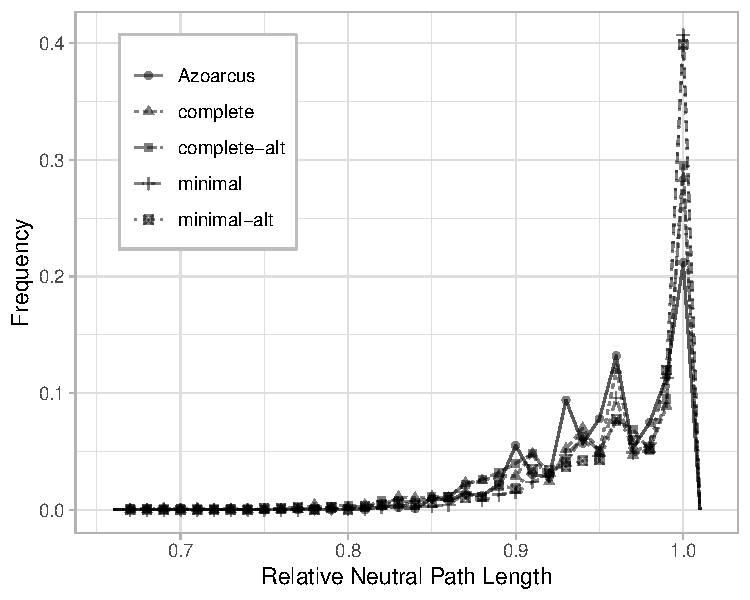
\includegraphics[width=\textwidth]{pic/results/designs/npaths/nprelative-freq-binwidth001.pdf}
	%	\caption{Bin width $=0.01$. Path lengths were normalized according to the total number of unpaired positions and base pairs \todo{effectively not as accurate as reduced strings, but what we are actually measuring is hamming distance which I saved}.
	%	}\label{fig:percolation:a}
	%\end{subfigure}%
	%\begin{subfigure}[t]{0.5\textwidth}
	%	\centering
	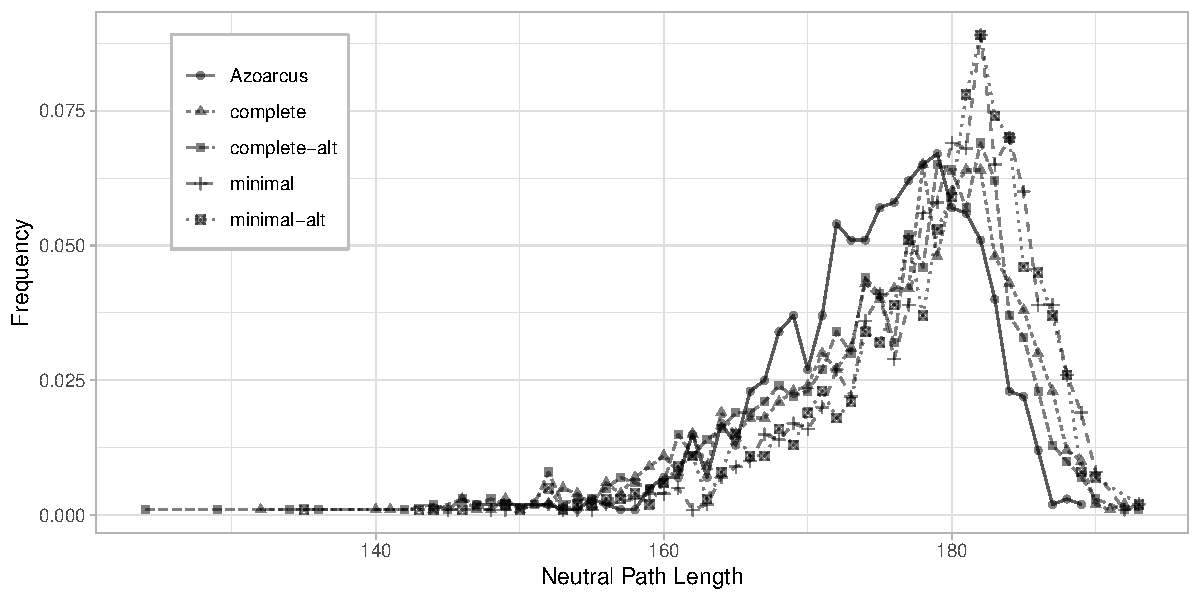
\includegraphics[width=\textwidth]{pic/results/designs/npaths/hamming-freq-wide.pdf}
	%	\caption{hamming distance between first and last sequence
	%	}\label{fig:percolation:b}
	%\end{subfigure}
	\caption[Neutral Path Lengths]{
		%\begin{enumerate*}[label={(\alph*)}, font={\bfseries}]
		%	\item x-values below 1 result from stopping early to save time as I wasn't exhaustively enumerating all neighbors (choosing without repitition, that is) but sampling uniformly to save (dev) time (and memory; let's face it --- I just was lazy and RNAblueprint was sufficiently easy and did the job). technically, max. value is also stopping early, but the approach with stopping at component number was hopeful because of \parencite{haslinger_rna_1999}: we would expect to perculate, let's just check, therefore we can stop early
		%	\item b
		%\end{enumerate*}
		Lengths of neutral paths, each starting from a designed sequence.
		The paths were generated on the sequence spaces compatible to the \texttt{pKiss}-predicted structure of the initial sequence.
		Neutral paths of the same length were counted and normalized by the number of designs per constraint set.
		See \autoref{tab:percolationstats} for the mean lengths of each constraint set.
		The generated paths starting from \textit{Azoarcus} were plotted slightly darker.
	}\label{fig:percolation}
\end{figure}

Overall, the distributions seem to be very similar.
The distribution for \texttt{Azoarcus} appears to be shifted slightly to the left, which is probably an artifact resulting from stopping the neutral paths early.
Still, the mean length of the computed neutral paths starting from \textit{Azoarcus} is very close to and within the standard deviation of the mean lengths computed for \texttt{complete} and \texttt{complete-alt} (\autoref{tab:percolationstats}).
Although slightly higher, the same statement applies to the mean lengths of \texttt{complete} and \texttt{complete-alt}.

\begin{table}[!ht]
	\centering\setstretch{0.95}
	\caption[Mean Neutral Path Lengths and Expected Random Hamming Distances]{
		Mean neutral path lengths of designed sequences and the expected Hamming distances between two random sequences compatible to the \texttt{pKiss}-predicted structure for each designed sequence per constraint set.
		The displayed values are mean values for each set including standard deviation.
		The expected Hamming distance of two random compatible sequences was estimated for each neutral structure as described in \autoref{sub:methods:neutral} (see \autoref{eq:expected_hamming}). 
		For \textit{Azoarcus}, the reference sequence was used as initial sequence and 1000 neutral paths were generated on the sequence space compatible to the structure predicted by \texttt{pKiss}.
	}
	\label{tab:percolationstats}
	\begin{tabularx}{\textwidth}{lXcc} \toprule
		\textbf{Set} ($n=1000$) && Neutral Path Length & Expected Hamming Distance \\ \midrule
		\texttt{minimal} && $ 178.90 \pm 6.90 $ & $ 144.47 \pm 0.13 $  \\
		\texttt{complete} && $ 175.66 \pm 8.67 $  & $ 144.50 \pm 0.12 $  \\
		\texttt{minimal-alt} && $ 178.10 \pm 7.83 $  & $ 144.52 \pm 0.17 $  \\
		\texttt{complete-alt} && $ 175.13 \pm 9.05 $  & $ 144.52 \pm 0.15 $  \\
		\midrule
		\textit{Azoarcus} && $ 174.97 \pm 6.55 $  & $ 144.36 \pm 0.00 $  \\ 
		\bottomrule
	\end{tabularx}
\end{table}

The mean expected Hamming distance of two random sequences compatible to the same structure is almost equal in the spaces of compatible sequences used for neutral path computation in each set (\autoref{tab:percolationstats}).
This observation is due to the overall design goal to produce structures similar to the \textit{Azoarcus} group I intron and the dependence of the expected Hamming distance on the number of unpaired positions and base pairs (see \autoref{eq:expected_hamming}).
Naturally, the standard deviation of the expected Hamming distance is equal to zero given the same predicted structure in all neutral paths for \textit{Azoarcus}.
It may be notable that in the sequence space compatible to the native structure (see \autoref{fig:azodata:b}), the expected distance between two random sequences is approximately $144.47$ ($u=79$, $b=59$).

Recalling \autoref{sub:methods:neutral}, it should be emphasized that the expected Hamming distance between to random compatible sequence is not a threshold for sequence space percolation but used to put the computed neutral length paths into perspective.
Furthermore, since  $\nicefrac{13}{18} \approx \nicefrac{3}{4}$, \autoref{eq:expected_hamming} is well approximated by the expected Hamming distance of two random sequences not necessarily compatible to a shared structure:  $\nicefrac{3}{4}\, N$ \parencite{haslinger_rna_1999}.

In summary, neutral paths of designed sequences do not reach maximum length but are still very long, indicating extended neutral networks of similar structures.
This is encouraging since neutral network size correlates with mutational robustness \parencite{jorg_neutral_2008} although this should be interpreted with care. 
The lower bound provided by neutral path lengths does not correspond to the number of sequences folding into a structure but rather how far-reaching the neutral network extends through sequence space.
If a designed RNA sequence proved to be functional, this would be a desirable property similar to results in the \textit{Azoargus} group I intron \parencite{hayden_intramolecular_2015}.

It has been previously shown that percolating neutral networks exist in spaces mapping RNA sequences (of length \unit[100]{nt}) to crossing secondary structures \parencite{haslinger_rna_1999}.
The results described here are aligned very well with the data in \parencite[Fig. 9]{haslinger_rna_1999}, even though a different mapping between sequences and structures was employed by using \texttt{pKiss}.
However, the generated neutral paths are not neutral to the actual target structure (\autoref{sub:theory:seqtargetstruct}).

\end{document}
